%!TEX TS-program = xelatex
%!en_GB
\documentclass[]{friggeri-cv}
\usepackage{afterpage}
\usepackage{array, booktabs}
\usepackage{hyperref}
\usepackage{color}
\usepackage{xcolor}
\usepackage{smartdiagram}
\usepackage{fontspec}
\usepackage{fontawesome} % you need to compile the tex file with LuaLaTeX
\usepackage{metalogo}
\usepackage{dtklogos}
\usepackage[utf8]{inputenc}
\usepackage{tikz}
\usetikzlibrary{mindmap,shadows}
\hypersetup{
    pdftitle={},
    pdfauthor={},
    pdfsubject={},
    pdfkeywords={},
    colorlinks=false,           % no lik border color
    allbordercolors=white       % white border color for all
}
\smartdiagramset{
    bubble center node font = \footnotesize,
    bubble node font = \footnotesize,
    % specifies the minimum size of the bubble center node
    bubble center node size = 0.5cm,
    %  specifies the minimum size of the bubbles
    bubble node size = 0.5cm,
    % specifies which is the distance among the bubble center node and the other bubbles
    distance center/other bubbles = 0.3cm,
    % sets the distance from the text to the border of the bubble center node
    distance text center bubble = 0.5cm,
    % set center bubble color
    bubble center node color = pblue,
    % define the list of colors usable in the diagram
    set color list = {lightgray, materialcyan, orange, green, materialorange, materialteal, materialamber, materialindigo, materialgreen, materiallime},
    % sets the opacity at which the bubbles are shown
    bubble fill opacity = 0.6,
    % sets the opacity at which the bubble text is shown
    bubble text opacity = 0.5,
}
\newcolumntype{L}[1]{>{\raggedright\let\newline\\\arraybackslash\hspace{0pt}}m{#1}}
\newcolumntype{C}[1]{>{\centering\let\newline\\\arraybackslash\hspace{0pt}}m{#1}}
\newcolumntype{R}[1]{>{\raggedleft\let\newline\\\arraybackslash\hspace{0pt}}m{#1}}
\RequirePackage{xcolor}
\definecolor{pblue}{HTML}{0395DE}

\begin{document}
\header{Gessica}{Trivelli}
      {Midwife}
      
% Fake text to add separator      
\fcolorbox{white}{gray}{\parbox{\textwidth-2\fboxsep-2\fboxrule}{%
.....
}}

% In the aside, each new line forces a line break
\begin{aside}
  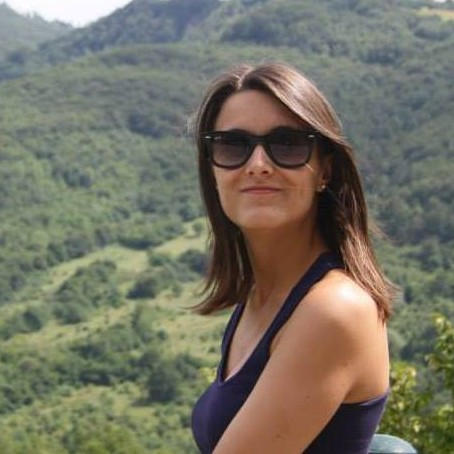
\includegraphics[width=4.2cm, keepaspectratio]{img/gessica_crop.jpg}
  ~
  ~
	\section{Address}
	68, Aldo Moro,
	Comunanza (AP), 63087, Italy
    ~
	\section{Tel \& Skype}
    +39 339 505 0697 \vspace{3pt}
    gessica.trivelli\\@gmail.com
    ~
	\section{Mail}
    \href{mailto:gessica.trivelli@gmail.com}{\textbf{gessica.trivelli@}\\gmail.com}
    ~
    \section{Personal Informations}
	\textbf{Nationality}: Italian
	\textbf{Birthday}: April 14 1991
	~
\end{aside}
\vspace{2.65cm}
\section{Education}
\begin{entrylist}
	\entry
	{2016 - Now}
	{Postgraduate Specialization in Midwifery [\small EQF 7]}
	{\\Scuola Elementale di Arte Ostetrica, Florence}
	{50 ECM Specialization Course - 194 hours - on the following topic: \emph{Pelvic floor's health in female cycle: education, prevention re-education and treatment of perineal dysfunction using a midwifery-led approach.}\\}
	
	\entry
	{2014 - Now}
	{Master's Degree in Nursing and Midwifery [\small EQF 7]}
	{\\Tor Vergata, University of Rome}
	{Graduation in March 2017. \\Internship - thesis at \textit{"Istituto Superiore di Sanita'"} on the following topic: \textit{Health knowledge, attitudes and practice of midwifery students, pregnant women and midwives on umbilical cord clamping and cord blood stem cells transplantation.}\\}
	
	\entry
	{2010 - 2014}
	{Bachelor's Degree in Midwifery [\small EQF 6]}
	{\\Tor Vergata, University of Rome}
	{First class with honors.\\
	Internship in Rome in several hospitals: \textit{Policlinico Tor Vergata}, \textit{Azienza Ospedaliera San Giovanni Addolorata}, \textit{Ospedale Fatebenefratelli San Giovanni Calibita} and \textit{Policlinico Casilino}.\\
	Thesis title: \textit{Survey on Women's Positions during Labour and Delivery: Evaluation of Maternal and Foetal Outcomes.}\\}

	\entry
	{2005-2010}
	{Scientific Diploma [\small EQF 4]}
	{\\Scientific High School "A. Gentili", Sarnano (MC)}
	{}
\end{entrylist}

\section{Experience}
\begin{entrylist}
  \entry
  {2015 - Now}
  {Collaborator}
  {\\CreAttivaMente Ostetriche}
  {Co-administrator of the blog \href{http://creattivamenteostetriche2012.blogspot.it/}{CreAttivaMente Ostetriche}. 
  	Secretaryship and ECM-course co-oragnisation.\\}
  
  \entry
    {2010 - 2010}
    {Volunteer}
    {\\Croce Rossa Italiana - Italian Commitee of Sibillini}
    {\\}
\end{entrylist}

\newpage
\begin{aside}
~
~
~
    % use  \hspace{} or \vspace{} to change bubble size, if needed
	\section{IT Skills}
	\textbf{macOS}
\includegraphics[scale=0.40]{img/5stars.png}
	\textbf{Windows}
\includegraphics[scale=0.40]{img/5stars.png}
	\textbf{Office}
\includegraphics[scale=0.40]{img/5stars.png}
	\textbf{iWork}
\includegraphics[scale=0.40]{img/4stars.png}
	\textbf{Epi-Info}
\includegraphics[scale=0.40]{img/3stars.png}
	\textbf{Pubmed}
\includegraphics[scale=0.40]{img/5stars.png}
	~
	\section{Relational Skills}
	Women-centred care,promoting information and free decision making, through skills such as \textbf{counselling}, \textbf{empathy} and \textbf{active listening}.
	~
	\section{Technical Skills}
	Problem solving
	~
	Use of brand new and innovative didactic models
	~
	Education in the adulthood
	~
	Planning, implementation and evaluation of clinical, organizational and pedagogical topics
	~
	Quantitative and qualitative research in clinical, organizational and pedagogical fields
	~
	Evaluation of care services (e.g. quality, pertinence, safety and cheapness)
\end{aside}


\section{Honours \& Awards}
\begin{entrylist}
	\entry
	{06/2016}
	{Tutoring scholarship}
	{\\Tor Vergata, University of Rome}
	{}
	{}
\end{entrylist}

\section{Certifications}
\begin{entrylist}
  \entry
	  {2016}
	  {Emergencies during delivery.}
	  {\\CreAttivaMente Ostetriche, Rome}
	  {16 hours course - using medical mannequin.\\}
  \entry
	  {2015}
	  {Advanced skills to support breastfeeding.}
	  {\\CreAttivaMente Ostetriche, Rome}
	  {16 hours course.\\}
  \entry
	  {2015}
	  {Management of infertility - education, information and communication in IVF.}
	  {\\Ministero della Salute}
	  {8 hours course.\\}
  \entry
  {2014}
  {Breastfeeding: counselling practical course, OMS/UNICEF model.}
  {\\Tor Vergata, University of Rome}
  {40 hours course.\\}
\end{entrylist}
\vspace{15pt}
\section{Languages}
\begin{table*}[!hf]
	\centering
	\renewcommand{\arraystretch}{1.45}
	\begin{tabular}{ C{2cm} C{3cm} C{3cm} C{3cm} }
		\toprule
		& \textbf{Writing} 	& \textbf{Speaking} & \textbf{Listening}			\\ 
		\midrule
		\textbf{Italian:}	& \multicolumn{3}{c}{Mother-tongue}					\\ 
		\textbf{English:} 	& B1 				& B1 			& B1			\\ 
		\textbf{French:}	& B1 				& B1			& B1			\\
		\bottomrule
	\end{tabular}
\end{table*}
\vspace{15pt}
\section{Other informations}
\begin{itemize}
	\item Currently subscribed to the \textit{Collegio Ostetriche di Roma - n. 2640}.
	\item \textit{Application Pack} from \textit{NMBI} - \textit{Nursing and Midwifery Board of Ireland} is currently pending.
\end{itemize}
\leavevmode\vspace{1.5cm}
\begin{flushleft}
\emph{\Large January 18th 2017}
\end{flushleft}
\begin{flushright}
\emph{\Large Gessica Trivelli}
\end{flushright}

\end{document}
